\section{Arc Length}{}{}\label{sec:Arc Length}


In previous sections we used integration to answer the following questions:
	\begin{enumerate}
	\item		Given a region, what is its area?
	\item		Given a solid, what is its volume?
	\end{enumerate}
	
In this section, we address a related question: Given a curve, what is its length? This is often referred to as \textbf{arc length}. 

Consider the graph of $y=\sin x$ on $[0,\pi]$ given in Figure \ref{fig:arcintro} (a). How long is this curve? That is, if we were to use a piece of string to exactly match the shape of this curve, how long would the string be?

As we have done in the past, we start by approximating; later, we will refine our answer using limits to get an exact solution.

The length of straight--line segments is easy to compute using the Distance Formula. We can approximate the length of the given curve by approximating the curve with straight lines and measuring their lengths. 


\begin{figure}[H]
	\centering
	\begin{subfigure}[t]{0.5\textwidth}
		\begin{tikzpicture}
		\begin{axis}[ width=\linewidth,%
		tick label style={font=\scriptsize},axis y line=middle,axis x line=middle,name=myplot,axis on top,%
					%x=.37\marginparwidth,
					%y=.37\marginparwidth,
					xtick=\empty,% 
					extra x ticks={.79,1.57,2.36,3.14},
					extra x tick labels={$\frac{\pi}4$,$\frac{\pi}2$,$\frac{3\pi}{4}$,$\pi$},
		%			ytick={1},
		%			yticklabels={$-0.002$,$0.002$,$0.004$},
					%minor y tick num=1,
		%			extra y ticks={1.8},%
		%			extra y tick labels={$y$},
		%			minor x tick num=4,
					ymin=-.2,ymax=1.25,%
					xmin=-.1,xmax=3.5,%
		]
		
		\addplot [{\colorone},smooth,thick,domain=0:3.14] {sin(deg(x))};
		
		\end{axis}
		
		\node [right] at (myplot.right of origin) {\scriptsize $x$};
		\node [above] at (myplot.above origin) {\scriptsize $y$};
		\end{tikzpicture}
         \label{fig:arcintroa}
        \caption{} 
    \end{subfigure}% 
    \begin{subfigure}[t]{0.5\textwidth}
    \begin{tikzpicture}
    \begin{axis}[ width=\linewidth,%
    tick label style={font=\scriptsize},axis y line=middle,axis x line=middle,name=myplot,axis on top,%
    			%x=.37\marginparwidth,
    			%y=.37\marginparwidth,
    			xtick=\empty,% 
    			extra x ticks={.79,1.57,2.36,3.14},
    			extra x tick labels={$\frac{\pi}4$,$\frac{\pi}2$,$\frac{3\pi}{4}$,$\pi$},
    %			ytick={1},
    %			yticklabels={$-0.002$,$0.002$,$0.004$},
    			%minor y tick num=1,
    			extra y ticks={.71},%
    			extra y tick labels={$\frac{\sqrt{2}}2$},
    %			minor x tick num=4,
    			ymin=-.2,ymax=1.25,%
    			xmin=-.1,xmax=3.5,%
    ]
    
    \addplot [{\colorone},smooth,thick,domain=0:3.14] {sin(deg(x))};
    
    \draw [{\colortwo},thick] (axis cs:0,0) -- (axis cs:.79,.71) -- (axis cs: 1.57,1) -- (axis cs:2.36,.71) -- (axis cs: 3.14,0);
    
    \filldraw (axis cs:0,0) circle (1pt) (axis cs:.79,.71) circle (1pt) (axis cs: 1.57,1) circle (1pt) (axis cs:2.36,.71) circle (1pt) (axis cs: 3.14,0)circle (1pt);
    
    \end{axis}
    
    \node [right] at (myplot.right of origin) {\scriptsize $x$};
    \node [above] at (myplot.above origin) {\scriptsize $y$};
    \end{tikzpicture}
        \label{fig:arcintrob}
        \caption{}    
    \end{subfigure} 
    \caption{Graphing $y=\sin x$ on $[0,\pi]$ and approximating the curve with line segments. \label{fig:arcintro}}
\end{figure}

In Figure \ref{fig:arcintro} (b), the curve $y=\sin x$ has been approximated with 4 line segments (the interval $[0,\pi]$ has been divided into 4 equally--lengthed subintervals). It is clear that these four line segments approximate $y=\sin x$ very well on the first and last subinterval, though not so well in the middle. Regardless, the sum of the lengths of the line segments is $3.79$, so we approximate the arc length of $y=\sin x$ on $[0,\pi]$ to be $3.79$. 

%Using 6 evenly spaced subintervals is not too much more work and gives a better approximation. The six lines are shown in Figure \ref{fig:arcintroc} and provide an arc length approximation of $3.81$. 

%\begin{figure}[H]
%\begin{tikzpicture}
%\begin{axis}[width=\marginparwidth+25pt,%
%tick label style={font=\scriptsize},axis y line=middle,axis x line=middle,name=myplot,axis on top,%
%			%x=.37\marginparwidth,
%			%y=.37\marginparwidth,
%			xtick=\empty,% 
%			extra x ticks={.52,1.05,1.6,2.1,2.6,3.14},
%			extra x tick labels={$\frac{\pi}6$,$\frac{\pi}3$,$\frac{\pi}{2}$,$\frac{2\pi}3$,$\frac{5\pi}6$,$\pi$},
%%			ytick={1},
%%			yticklabels={$-0.002$,$0.002$,$0.004$},
%			%minor y tick num=1,
%			extra y ticks={.866},%
%			extra y tick labels={$\frac{\sqrt{3}}2$},
%%			minor x tick num=4,
%			ymin=-.2,ymax=1.25,%
%			xmin=-.1,xmax=3.5,%
%]
%
%\addplot [{\colorone},smooth,thick,domain=0:3.14] {sin(deg(x))};
%
%\draw [{\colortwo},thick] (axis cs:0,0)--(axis cs:0.5236,0.5)--(axis cs:1.047,0.866)--(axis cs:1.571,1.)--(axis cs:2.094,0.866)--(axis cs:2.618,0.5)--(axis cs:3.142,0);
%
%\filldraw (axis cs:0,0) circle (1pt) (axis cs:0.5236,0.5) circle (1pt) (axis cs:1.047,0.866) circle (1pt) (axis cs:1.571,1.) circle (1pt) (axis cs:2.094,0.866) circle (1pt) (axis cs:2.618,0.5) circle (1pt) (axis cs:3.142,0);
%
%\end{axis}
%
%\node [right] at (myplot.right of origin) {\scriptsize $x$};
%\node [above] at (myplot.above origin) {\scriptsize $y$};
%\end{tikzpicture}
%\label{fig:arcintroc}
%\end{figure}



In general,  we can approximate the arc length of $y=f(x)$ on $[a,b]$ in the following manner. Let $a=x_1 < x_2 < \ldots < x_n< x_{n+1}=b$ be a partition of $[a,b]$ into $n$ subintervals. Let $\dx_i$ represent the length of the $i\,^\text{th}$ subinterval $[x_i,x_{i+1}]$.

\begin{figure}[H]
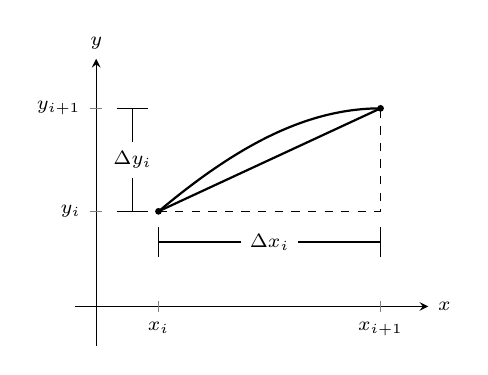
\begin{tikzpicture}
\begin{axis}[width=.5\linewidth,%
tick label style={font=\scriptsize},axis y line=middle,axis x line=middle,name=myplot,axis on top,%
			%x=.37\marginparwidth,
			%y=.37\marginparwidth,
			xtick=\empty,% 
			extra x ticks={.3,1.37},
			extra x tick labels={$x_i$,$x_{i+1}$},
			ytick=\empty,
%			yticklabels={$-0.002$,$0.002$,$0.004$},
			%minor y tick num=1,
			extra y ticks={.48,1},%
			extra y tick labels={$y_i$,$y_{i+1}$},
%			minor x tick num=4,
			ymin=-.2,ymax=1.25,%
			xmin=-.1,xmax=1.6,%
]
%\addplot [{\colorone},smooth,thin,dashed,domain=0.1:1.55] {sin(deg(x+.2))};

\addplot [{\colorone},smooth,thick,domain=0.3:1.37] {sin(deg(x+.2))};

\draw (axis cs: .25,1) -- (axis cs:.1,1) 
			(axis cs: .25,.48) -- (axis cs:.1,.48)
			(axis cs: .175,.48) -- node [pos=.5,fill=white] {\scriptsize $\Delta y_i$} (axis cs:.175,1);

\draw (axis cs: .3,.25) -- (axis cs: .3,.4)
			(axis cs: 1.37,.25) -- (axis cs: 1.37,.4)
			(axis cs: .3,.325) -- node [pos=.5,fill=white] {\scriptsize $\Delta x_i$} (axis cs: 1.37,.325);
			
\draw [{\colortwo},thick] (axis cs: .3,.48) -- (axis cs:1.37,1);

\draw [dashed,thin] (axis cs: .3,.48) -| (axis cs:1.37,1);
			
\filldraw (axis cs: .3,.48) circle (1pt) (axis cs:1.37,1) circle (1pt);

%\draw [{\colortwo},thick] (axis cs:0,0)--(axis cs:0.5236,0.5)--(axis cs:1.047,0.866)--(axis cs:1.571,1.)--(axis cs:2.094,0.866)--(axis cs:2.618,0.5)--(axis cs:3.142,0);
%
%\filldraw (axis cs:0,0) circle (1pt) (axis cs:0.5236,0.5) circle (1pt) (axis cs:1.047,0.866) circle (1pt) (axis cs:1.571,1.) circle (1pt) (axis cs:2.094,0.866) circle (1pt) (axis cs:2.618,0.5) circle (1pt) (axis cs:3.142,0);

\end{axis}

\node [right] at (myplot.right of origin) {\scriptsize $x$};
\node [above] at (myplot.above origin) {\scriptsize $y$};
\end{tikzpicture}
\label{fig:arcintro2}
\caption{Zooming in on the $i\,^\text{th}$ subinterval $[x_i,x_{i+1}$] of a partition of $[a,b]$.}
\end{figure}


%\mfigure{.35}{Zooming in on the $i\,^\text{th}$ subinterval $[x_i,x_{i+1}$] of a partition of $[a,b]$.}{fig:arcintro2}{figures/figarcintrod}
%
Figure \ref{fig:arcintro2} zooms in on the $i\,^\text{th}$ subinterval where $y=f(x)$ is approximated by a straight line segment. The dashed lines show that we can view this line segment as they hypotenuse of a right triangle whose sides have length $\dx_i$ and $\dy_i$. Using the Pythagorean Theorem, the length of this line segment is
$\ds \sqrt{\dx_i^2 + \Delta y_i^2}.$ Summing over all subintervals gives an arc length approximation
$$L \approx \sum_{i=1}^n \sqrt{\dx_i^2 + \Delta y_i^2}.$$

As shown here, this is \textit{not} a Riemann Sum. While we could conclude that taking a limit as the subinterval length goes to zero gives the exact arc length, we would not be able to compute the answer with a definite integral. We need first to do a little algebra.

In the above expression factor out a $\dx_i^2$ term:
\begin{align*}
\sum_{i=1}^n \sqrt{\dx_i^2 + \Delta y_i^2} &= \sum_{i=1}^n \sqrt{\dx_i^2\left(1 + \frac{\Delta y_i^2}{\dx_i^2}\right)}.\\
\intertext{Now pull the $\dx_i^2$ term out of the square root:}%\\
			&= \sum_{i=1}^n\sqrt{1 + \frac{\Delta y_i^2}{\dx_i^2}}\ \dx_i.\\
\intertext{This is nearly a Riemann Sum. Consider the $\Delta y_i^2/\dx_i^2$ term. The expression $\Delta y_i/\dx_i$ measures the ``change in $y$/change in $x$,'' that is, the ``rise over run'' of $f$ on the $i\,^\text{th}$ subinterval. The Mean Value Theorem of Differentiation (Theorem \ref{thm:mvt}) states that there is a $c_i$ in the $i\,^\text{th}$ subinterval where $\fp(c_i) = \Delta y_i/\dx_i$. Thus we can rewrite our above expression as:} 
			&= \sum_{i=1}^n\sqrt{1+\fp(c_i)^2}\ \dx_i.\\
\intertext{This \textit{is} a Riemann Sum. As long as \fp\ is continuous, we can invoke Theorem \ref{thm:riemann_sum} and conclude }%\\
			&= \int_a^b\sqrt{1+\fp(x)^2}\ dx.
\end{align*}


\begin{formulabox}[\label{idea:arclength} Arc Length ]
{Let $f$ be differentiable on an open interval containing $[a,b]$, where $\fp$ is also continuous on $[a,b]$. Then the arc length of $f$ from $x=a$ to $x=b$ is
\index{integration!arc length}\index{arc length}
$$L = \int_a^b \sqrt{1+\fp(x)^2}\ dx.$$
}

\end{formulabox}


As the integrand contains a square root, it is often difficult to use the formula in Key Idea \ref{idea:arclength} to find the length exactly. When exact answers are difficult to come by, we resort to using numerical methods of approximating definite integrals. The following examples will demonstrate this.\\


\begin{example}{Finding arc length}{ex_arc1}
{
Find the arc length of $f(x) = x^{3/2}$ from $x=0$ to $x=4$. }
\end{example}


\begin{solution}
{We begin by finding $\fp(x)= \frac32x^{1/2}$. Using the formula, we find the arc length $L$ as
\begin{align*}
	L &=	\int_0^4 \sqrt{1+\left(\frac32x^{1/2}\right)^2}\ dx \\
		&=	\int_0^4 \sqrt{1+\frac94x} \ dx \\
		&= 	\int_0^4 \left(1+\frac94x\right)^{1/2}\ dx \\
		&=  \frac23\frac49\left(1+\frac94x\right)^{3/2}\Big|_0^4 \\
		&=\frac{8}{27}\left(10^{3/2}-1\right) \approx 9.07 \text{units}.
\end{align*}

\begin{figure}[H]
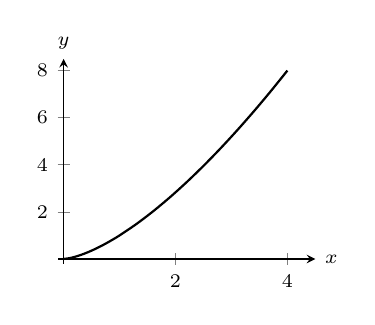
\begin{tikzpicture}
\begin{axis}[width=.4\linewidth,%
tick label style={font=\scriptsize},axis y line=middle,axis x line=middle,name=myplot,axis on top,%
			%x=.37\marginparwidth,
			%y=.37\marginparwidth,
%			xtick=\empty,% 
%			extra x ticks={.79,1.57,2.36,3.14},
%			extra x tick labels={$\frac{\pi}4$,$\frac{\pi}2$,$\frac{3\pi}{4}$,$\pi$},
%			ytick={1},
%			yticklabels={$-0.002$,$0.002$,$0.004$},
			%minor y tick num=1,
%			extra y ticks={1.8},%
%			extra y tick labels={$y$},
%			minor x tick num=4,
			ymin=-.2,ymax=8.5,%
			xmin=-.1,xmax=4.5,%
]

\addplot [{\colorone},smooth,thick,domain=0:4,samples=50] coordinates {(0,0)(0.1,0.03162)(0.2,0.08944)(0.3,0.1643)(0.4,0.253)(0.5,0.3536)(0.6,0.4648)(0.7,0.5857)(0.8,0.7155)(0.9,0.8538)(1.,1.)(1.3,1.482)(1.6,2.024)(1.9,2.619)(2.2,3.263)(2.5,3.953)(2.8,4.685)(3.1,5.458)(3.4,6.269)(3.7,7.117)(4.,8.)};

\end{axis}

\node [right] at (myplot.right of origin) {\scriptsize $x$};
\node [above] at (myplot.above origin) {\scriptsize $y$};
\end{tikzpicture}
\caption{A graph of $f(x) = x^{3/2}$ from Example \ref{exa:ex_arc1}. \label{fig:arc1}}
\end{figure}
}
\end{solution}



\begin{example}{Finding arc length}{ex_arc2}{
Find the arc length of $\ds f(x) =\frac18x^2-\ln x$ from $x=1$ to $x=2$.}
\end{example}


\begin{solution}
{This function was chosen specifically because the resulting integral can be evaluated exactly. We begin by finding $\fp(x) = x/4-1/x$. The arc length is 
\begin{align*}
L		&=  \int_1^2 \sqrt{1+ \left(\frac x4-\frac1x\right)^2}\ dx \\
		&= 	\int_1^2 \sqrt{1 + \frac{x^2}{16} -\frac12 + \frac1{x^2} } \ dx \\
		&=	\int_1^2 \sqrt{\frac{x^2}{16} +\frac12 + \frac1{x^2} } \ dx \\
		&=	\int_1^2	\sqrt{ \left(\frac x4 + \frac1x\right)^2}\ dx 
\end{align*}
\begin{align*}
\phantom{L}
				&= \int_1^2 \left(\frac x4 + \frac1x\right) \ dx \\
		&=  \left(\frac{x^2}8 + \ln x\right)\Bigg|_1^2\\
		&=	\frac38+\ln 2 \approx 1.07 \ \text{units}.
\end{align*}

\begin{figure}[H]
\begin{tikzpicture}
\begin{axis}[width=.4\linewidth,%
tick label style={font=\scriptsize},axis y line=middle,axis x line=middle,name=myplot,axis on top,%
			%x=.37\marginparwidth,
			%y=.37\marginparwidth,
%			xtick=\empty,% 
%			extra x ticks={.79,1.57,2.36,3.14},
%			extra x tick labels={$\frac{\pi}4$,$\frac{\pi}2$,$\frac{3\pi}{4}$,$\pi$},
%			ytick={1},
%			yticklabels={$-0.002$,$0.002$,$0.004$},
			%minor y tick num=1,
%			extra y ticks={1.8},%
%			extra y tick labels={$y$},
%			minor x tick num=4,
			ymin=-.26,ymax=1.2,%
			xmin=-.1,xmax=3.1,%
]
\addplot [{\colorone},smooth,thin] coordinates{(0.2,1.614)(0.3,1.215)(0.4,0.9363)(0.5,0.7244)(0.6,0.5558)(0.7,0.4179)(0.8,0.3031)(0.9,0.2066)(1.,0.125)(1.1,0.05594)(1.2,-0.002322)(1.3,-0.05111)(1.4,-0.09147)(1.5,-0.1242)(1.6,-0.15)(1.7,-0.1694)(1.8,-0.1828)(1.9,-0.1906)(2.,-0.1931)(2.1,-0.1907)(2.2,-0.1835)(2.3,-0.1717)(2.4,-0.1555)(2.5,-0.135)(2.6,-0.1105)(2.7,-0.082)(2.8,-0.04962)(2.9,-0.01346)(3.,0.02639)};

\addplot [{\colorone},smooth,very thick,] coordinates {(1.,0.125)(1.1,0.05594)(1.2,-0.002322)(1.3,-0.05111)(1.4,-0.09147)(1.5,-0.1242)(1.6,-0.15)(1.7,-0.1694)(1.8,-0.1828)(1.85,-0.1874)(1.9,-0.1906)(1.95,-0.1925)(2.,-0.1931)};


\end{axis}

\node [right] at (myplot.right of origin) {\scriptsize $x$};
\node [above] at (myplot.above origin) {\scriptsize $y$};
\end{tikzpicture}
\caption{A graph of $f(x) =\frac18x^2-\ln x$ from Example \ref{ex_arc2}. \label{fig:arc2}}
\end{figure}

A graph of $f$ is given in Figure \ref{fig:arc2}; the portion of the curve measured in this problem is in bold.
}
\end{solution}


\begin{example}{Circumference of a Circle}{Circumference of a Circle}\label{Circumference of a Circle} 
Let $\ds f(x) = \sqrt{r^2-x^2}$, the upper half circle of radius
$r$. The length of this curve is half the circumference, namely $\pi
r$. Compute this with the arc length formula.
\end{example}

\begin{solution}
The derivative $f'$ is $\ds \ds -x/\sqrt{r^2-x^2}$ so the integral is
$$
  \int_{-r}^r \sqrt{1+{x^2\over r^2-x^2}}\,dx
  =\int_{-r}^r \sqrt{r^2\over r^2-x^2}\,dx
  =r\int_{-r}^r \sqrt{1\over r^2-x^2}\,dx.
$$
Using a trigonometric substitution, we find the antiderivative, namely
$\ds \arcsin(x/r)$. Notice that the integral is improper at both
endpoints, as the function $\ds \sqrt{1/(r^2-x^2)}$ is undefined when
$x=\pm r$. So we need to compute
$$
  \lim_{D\to-r^+}\int_D^0  \sqrt{1\over r^2-x^2}\,dx +
  \lim_{D\to r^-}\int_0^D  \sqrt{1\over r^2-x^2}\,dx.
$$
This is not difficult, and has value $\pi$, so the original integral,
with the extra $r$ in front, has value $\pi r$ as expected.
\end{solution}

The previous examples found the arc length exactly through careful choice of the functions. In general, exact answers are much more difficult to come by and numerical approximations are necessary. \\


\begin{example}{Approximating arc length numerically}{ex_arc3}
{
Find the length of the sine curve from $x=0$ to $x=\pi$.}
\end{example}


\begin{solution}
{This is somewhat of a mathematical curiosity; in Example \ref{ex_ftc4} we found the area under one ``hump'' of the sine curve is 2 square units; now we are measuring its arc length.

The setup is straightforward: $f(x) = \sin x$ and $\fp(x) = \cos x$. Thus 
$$L = \int_0^\pi \sqrt{1+\cos^2x}\ dx.$$
This integral \textit{cannot} be evaluated in terms of elementary functions so we will approximate it with Simpson's Method with $n=4$. 
\mtable{.5}{A table of values of $y=\sqrt{1+\cos^2x}$ to evaluate a definite integral in Example \ref{ex_arc3}.}{fig:arc3}{%
$$\begin{array}{cc}
x & \sqrt{1+\cos^2x} \\ \hline
 0 & \sqrt{2} \rule{0pt}{10pt}\\
 \pi/4 & \sqrt{3/2} \\
 \pi/2 & 1 \\
 3 \pi/4 & \sqrt{3/2} \\
 \pi  & \sqrt{2} \\
\end{array}$$
}
Figure \ref{fig:arc3} gives $\sqrt{1+\cos^2x}$ evaluated at 5 evenly spaced points in $[0,\pi]$. Simpson's Rule then states that 
\begin{align*}
\int_0^\pi \sqrt{1+\cos^2x}\ dx &\approx	\frac{\pi-0}{4\cdot 3}\left(\sqrt{2}+4\sqrt{3/2}+2(1)+4\sqrt{3/2}+\sqrt{2}\right) \\
			&=3.82918.
\end{align*}
Using a computer with $n=100$ the approximation is $L\approx 3.8202$; our approximation with $n=4$ is quite good.
}
\end{solution}




















% % % % % % % % % % % % % % % % % % % % % % % % % % % % % % % % % % % % % % % % % % % % % % %


%Here is another geometric application of the integral: Find the length
%of a portion of a curve. As usual, we need to think about how we might
%approximate the length, and turn the approximation into an integral.
%
%We already know how to compute one simple arc length, that of a line
%segment. If the endpoints are $\ds P_0(x_0,y_0)$ and $\ds P_1(x_1,y_1)$
%then the length of the segment is the distance between the points,
%$\ds \sqrt{(x_1-x_0)^2+(y_1-y_0)^2}$, from the Pythagorean theorem, as
%illustrated in Figure~\ref{fig:length of a line segment}.
%
%\figure[H]
%%\texonly
%\centerline{\vbox{\beginpicture
%\normalgraphs
%%\sevenpoint
%\setcoordinatesystem units <1.5truecm,1.5truecm>
%\setplotarea x from 0 to 5, y from 0 to 3
%\axis bottom /
%\axis left /
%\putrule from 2 1 to 4.5 1
%\putrule from 4.5 1 to 4.5 2.5
%\plot 2 1 4.5 2.5 /
%\put {$(x_1,y_1)$} [bl] <3pt,3pt> at 4.5 2.5
%\put {$(x_0,y_0)$} [tr] <-3pt,-3pt> at 2 1
%\put {$x_1-x_0$} [t] <0pt,-3pt> at 3.25 1
%\put {$y_1-y_0$} [l] <3pt,0pt> at 4.5 1.75
%\put {$\sqrt{(x_1-x_0)^2+(y_1-y_0)^2}$} [br] <-3pt,3pt> at 3.25 1.75
%\endpicture}}
%%\endtexonly
%%\figrdef{fig:length of a line segment}
%%\htmlfigure{Integration_applications-arc_length.html}
%\caption{\label{fig:length of a line segment}
%The length of a line segment.}
%%\endcaption
%\endfigure
%
%Now if the graph of $f$ is ``nice'' (say, differentiable) it appears
%that we can approximate the length of a portion of the curve with line
%segments, and that as the number of segments increases, and their
%lengths decrease, the sum of the lengths of the line segments will
%approach the true arc length; see 
%Figure~\ref{fig:approximating arc length}.
%
%\figure[H]
%%\texonly
%\centerline{\vbox{\beginpicture
%\normalgraphs
%%\sevenpoint
%\setcoordinatesystem units <1.5truecm,0.8truecm>
%\setplotarea x from 0 to 8, y from 0 to 5
%\axis bottom /
%\axis left /
%\setquadratic\plot 
%1.000 1.000 1.150 1.953 1.300 2.694 1.450 3.246 1.600 3.636 
%1.750 3.884 1.900 4.012 2.050 4.041 2.200 3.990 2.350 3.874 
%2.500 3.711 2.650 3.515 2.800 3.299 2.950 3.075 3.100 2.853 
%3.250 2.644 3.400 2.454 3.550 2.290 3.700 2.157 3.850 2.060 
%4.000 2.000 4.150 1.979 4.300 1.996 4.450 2.050 4.600 2.138 
%4.750 2.255 4.900 2.396 5.050 2.554 5.200 2.721 5.350 2.886 
%5.500 3.039 5.650 3.168 5.800 3.258 5.950 3.294 6.100 3.261 
%6.250 3.140 6.400 2.912 6.550 2.556 6.700 2.051 6.850 1.374 
%7.000 0.500 /
%\multiput {$\bullet$} at 1 1 2.050 4.041 3.250 2.644
%4.300 1.996 5.500 3.039 6.250 3.140 7 0.5 /
%\setlinear\plot
%1 1 2.050 4.041 3.250 2.644
%4.300 1.996 5.500 3.039 6.250 3.140 7 0.5 /
%\endpicture}}
%%\endtexonly
%%\figrdef{fig:approximating arc length}
%%\htmlfigure{Integration_applications-arc_length_line_segments.html}
%\caption{\label{fig:approximating arc length}
%Approximating arc length with line segments.}
%%\endcaption
%\endfigure
%
%Now we need to write a formula for the sum of the lengths of the line
%segments, in a form that we know becomes an integral in the limit.  So
%we suppose we have divided the interval $[a,b]$ into $n$ subintervals
%as usual, each with length $\Delta x =(b-a)/n$, and endpoints $\ds
%a=x_0$, $\ds x_1$, $\ds x_2$, \dots, $\ds x_n=b$.  The length of a
%typical line segment, joining $\ds (x_i,f(x_i))$ to $\ds
%(x_{i+1},f(x_{i+1}))$, is $\ds\sqrt{(\Delta x )^2
%  +(f(x_{i+1})-f(x_i))^2}$.  By the Mean Value Theorem, %(\xrefn{thm:mvt}), 
%there is a number $\ds t_i$ in $\ds (x_i,x_{i+1})$
%such that $\ds f'(t_i)\Delta x=f(x_{i+1})-f(x_i)$, so the length of
%the line segment can be written as
%$$
%  \sqrt{(\Delta x)^2 + (f'(t_i))^2\Delta x^2}=
%  \sqrt{1+(f'(t_i))^2}\,\Delta x.
%$$
%Then arc length is:
%$$
%  \lim_{n\to\infty}\sum_{i=0}^{n-1} \sqrt{1+(f'(t_i))^2}\,\Delta x=
%  \int_a^b \sqrt{1+(f'(x))^2}\,dx.
%$$
%Note that the sum looks a bit different than others we have
%encountered, because the approximation contains a $\ds t_i$ instead of an
%$\ds x_i$. In the past we have always used left endpoints (namely, $\ds x_i$)
%to get a representative value of $f$ on $\ds [x_i,x_{i+1}]$; now we are
%using a different point, but the principle is the same.
%
%To summarize, to compute the length of a curve on the interval
%$[a,b]$, we compute the integral
%$$\int_a^b \sqrt{1+(f'(x))^2}\,dx.$$ 
%Unfortunately, integrals of this form are typically difficult or
%impossible to compute exactly, because usually none of our methods for
%finding antiderivatives will work. In practice this means that the
%integral will usually have to be approximated.
%
%\begin{example}{Circumference of a Circle}{Circumference of a Circle}\label{Circumference of a Circle} 
%Let $\ds f(x) = \sqrt{r^2-x^2}$, the upper half circle of radius
%$r$. The length of this curve is half the circumference, namely $\pi
%r$. Compute this with the arc length formula.
%\end{example}
%
%\begin{solution}
%The derivative $f'$ is $\ds \ds -x/\sqrt{r^2-x^2}$ so the integral is
%$$
%  \int_{-r}^r \sqrt{1+{x^2\over r^2-x^2}}\,dx
%  =\int_{-r}^r \sqrt{r^2\over r^2-x^2}\,dx
%  =r\int_{-r}^r \sqrt{1\over r^2-x^2}\,dx.
%$$
%Using a trigonometric substitution, we find the antiderivative, namely
%$\ds \arcsin(x/r)$. Notice that the integral is improper at both
%endpoints, as the function $\ds \sqrt{1/(r^2-x^2)}$ is undefined when
%$x=\pm r$. So we need to compute
%$$
%  \lim_{D\to-r^+}\int_D^0  \sqrt{1\over r^2-x^2}\,dx +
%  \lim_{D\to r^-}\int_0^D  \sqrt{1\over r^2-x^2}\,dx.
%$$
%This is not difficult, and has value $\pi$, so the original integral,
%with the extra $r$ in front, has value $\pi r$ as expected.
%\end{solution}


%%%%%%%%%%%%%%%%%%%%%%%%%%%%%%%%%%%%%%%%%%%%
\Opensolutionfile{solutions}[ex]
\section*{Exercises for \ref{sec:Arc Length}}

\begin{enumialphparenastyle}

% % % % % % % % % % %
\begin{ex}
Find the arc length of the function on the given interval.
\begin{enumerate}
\item {$\ds f(x) = x$ on $[0, 1]$.}


\item {$\ds f(x) = \sqrt{8}x$ on $[-1, 1]$.}


\item {$\ds f(x) = \frac13x^{3/2}-x^{1/2}$ on $[0,1]$.}

\item {$\ds f(x) = \frac1{12}x^{3}+\frac1x$ on $[1,4]$.}


\item {$\ds f(x) = 2x^{3/2}-\frac16\sqrt{x}$ on $[0,9]$.}


\item {$\ds f(x) = \cosh x$ on $[-\ln 2, \ln 2]$.}


\item {$\ds f(x) = \frac12\big(e^x+e^{-x}\big)$ on $[0, \ln 5]$.}


\item {$\ds f(x) = \frac1{12}x^5+\frac1{5x^3}$ on $[.1, 1]$.}


\item {$\ds f(x) = \ln \big(\sin x\big)$ on $[\pi/6, \pi/2]$.}


\item {$\ds f(x) = \ln \big(\cos x\big)$ on $[0, \pi/4]$.}

\end{enumerate}

\begin{sol}
\begin{enumerate}
\item {$\sqrt{2}$}
\item {$6$}
\item {$4/3$}
\item {$6$}
\item {$109/2$}
\item {$3/2$}
\item {$12/5$}
\item {$79953333/400000 \approx 199.883$}
\item {$-\ln (2-\sqrt{3}) \approx 1.31696$}
\item {$\sinh^{-1} 1$}
\end{enumerate}
\end{sol}

\end{ex}
% % % % % % % % % % % %

% % % % % % % % % % %
\begin{ex}
Set up the integral to compute the arc length of the function on the given interval. Do \textbf{not} evaluate the integral. \label{ex_al1}
\begin{enumerate}
\item {$\ds f(x) = x^2$ on $[0, 1]$.\label{ex_07_04_ex_13}}


\item {$\ds f(x) = x^{10}$ on $[0, 1]$.}


\item {$\ds f(x) = \ln x$ on $[1, e]$.}


\item {$\ds f(x) = \sqrt{x}$ on $[0, 1]$.}


\item {$\ds f(x) = \sqrt{1-x^2}$ on $[-1, 1]$. (Note: this describes the top half of a circle with radius 1.)}


\item {$\ds f(x) = \sqrt{1-x^2/9}$ on $[-3, 3]$. (Note: this describes the top half of an ellipse with a major axis of length $ 6 $ and a minor axis of length $ 2 $.)}
\item {$\ds f(x) = \frac1x$ on $[1,2]$.}

\item {$\ds f(x) = \sec x$ on $[-\pi/4,\pi/4]$.\label{ex_07_04_ex_20}}

\end{enumerate}

\begin{sol}
\begin{enumerate}
\item {$\int_0^1 \sqrt{1+4x^2}\ dx$}
\item {$\int_0^1 \sqrt{1+100x^{18}}\ dx$}
\item {$\int_1^e \sqrt{1+\frac1{x^2}}\ dx$}
\item {$\int_0^1 \sqrt{1+\frac{1}{4x}}\ dx$}
\item {$\int_{-1}^1 \sqrt{1+\frac{x^2}{1-x^2}}\ dx$}
\item 
{$\int_{-3}^3 \sqrt{1+\frac{x^2}{81-9x^2}}\ dx$}

\item {$\int_{1}^2 \sqrt{1+\frac1{x^4}}\ dx$}
\item {$\int_{-\pi/4}^{\pi/4} \sqrt{1+\sec^2x\tan^2x}\ dx$}

\end{enumerate}
\end{sol}

\end{ex}
% % % % % % % % % % % %





% % % % % % % % % % %
\begin{ex}
Use Simpson's Rule, with $n=4$, to approximate the arc length of each the function on the given interval in Exercise \ref{ex_al1}. 

\begin{sol}
\begin{enumerate}
\item {$1.4790$}
\item {$1.8377$}
\item {$2.1300$}
\item 
\item 
\item 
\item {$1.4058$}
\item {$1.7625$}
\end{enumerate}
\end{sol}

\end{ex}
% % % % % % % % % % % %







%%%%%%%%%%
\begin{ex}
 Find the arc length of $\ds f(x)=x^{3/2}$ on $[0,2]$.
\begin{sol}
 $\ds (22\sqrt{22}-8)/27$
\end{sol}
\end{ex}

%%%%%%%%%%
\begin{ex}
 Find the arc length of $\ds f(x) = x^2/8-\ln x$
on $[1,2]$.
\begin{sol}
 $\ln(2)+3/8$
\end{sol}
\end{ex}

%%%%%%%%%%
\begin{ex}

Find the arc length of $\ds f(x) = (1/3)(x^2 +2)^{3/2}$
on the interval $[0,a]$.
\begin{sol}
 $\ds a+a^3/3$
\end{sol}
\end{ex}

%%%%%%%%%%
\begin{ex}
 Find the arc length of $f(x)=\ln(\sin x)$ on the
interval $[\pi/4,\pi/3]$.
\begin{sol}
 $\ds \ln((\sqrt2+1)/\sqrt3)$
\end{sol}
\end{ex}

%%%%%%%%%%
\begin{ex}
 Let $a>0$. Show that the length of $y=\cosh x$ on
$[0,a]$ is equal to $\ds \int _0 ^a \cosh x\,dx$.
\end{ex}

%%%%%%%%%%
\begin{ex}
 Find the arc length of $f(x)=\cosh x$ on $[0, \ln 2]$.
\begin{sol}
 $3/4$
\end{sol}
\end{ex}

%%%%%%%%%%
\begin{ex}
 Set up the integral to find the arc length of $\sin x$ 
on the interval $[0,\pi]$; do not evaluate the integral. If you have
access to appropriate software, approximate the value of the integral.
\begin{sol}
 $\approx 3.82$
\end{sol}
\end{ex}

%%%%%%%%%%
\begin{ex}
 Set up the integral to find the arc length of $\ds y=xe^{-x}$
on the interval $[2,3]$; do not evaluate the integral. If you have
access to appropriate software, approximate the value of the integral.
\begin{sol}
 $\approx 1.01$
\end{sol}
\end{ex}

%%%%%%%%%%
\begin{ex}
 Find the arc length of $\ds y=e^x$ on the interval $[0,1]$.
(This can be done exactly; it is a bit tricky and a bit long.)
\begin{sol}
 $\ds \sqrt{1+e^2}-\sqrt2+
{1\over2}\ln\left({\sqrt{1+e^2}-1\over\sqrt{1+e^2}+1}\right)+
{1\over2}\ln(3+2\sqrt2)$
\end{sol}
\end{ex}

\end{enumialphparenastyle}